\documentclass[tikz,border=8pt]{standalone}
% Shared look for every TikZ diagram. Load with % Shared look for every TikZ diagram. Load with % Shared look for every TikZ diagram. Load with \input{../../tools/tikz-style.tex}
\usepackage[T1]{fontenc}
\usepackage{lmodern}
\renewcommand{\sfdefault}{lmr}  % diagrams use the same serif as the text
\usetikzlibrary{arrows.meta, positioning, shapes.geometric, calc, fit, backgrounds}
\definecolor{cblue}{HTML}{4C78A8}
\definecolor{corange}{HTML}{F58518}
\definecolor{cgreen}{HTML}{54A24B}
\definecolor{cred}{HTML}{E45756}
\definecolor{cpurple}{HTML}{B279A2}
\definecolor{cgrey}{HTML}{6B6B6B}
\tikzset{
  every picture/.style={font=\sffamily, line width=1.2pt},
  box/.style={draw=#1, fill=#1!12, rounded corners=4pt, align=center, inner sep=7pt, minimum height=1.1cm},
  box/.default=cgrey,
  arrow/.style={-{Stealth[length=3mm]}, draw=cgrey, line width=1.4pt},
  title/.style={font=\sffamily\bfseries\Large},
  note/.style={font=\sffamily\small, text=cgrey, align=center},
}
\AtBeginDocument{\hyphenpenalty=10000 \exhyphenpenalty=10000}

\usepackage[T1]{fontenc}
\usepackage{lmodern}
\renewcommand{\sfdefault}{lmr}  % diagrams use the same serif as the text
\usetikzlibrary{arrows.meta, positioning, shapes.geometric, calc, fit, backgrounds}
\definecolor{cblue}{HTML}{4C78A8}
\definecolor{corange}{HTML}{F58518}
\definecolor{cgreen}{HTML}{54A24B}
\definecolor{cred}{HTML}{E45756}
\definecolor{cpurple}{HTML}{B279A2}
\definecolor{cgrey}{HTML}{6B6B6B}
\tikzset{
  every picture/.style={font=\sffamily, line width=1.2pt},
  box/.style={draw=#1, fill=#1!12, rounded corners=4pt, align=center, inner sep=7pt, minimum height=1.1cm},
  box/.default=cgrey,
  arrow/.style={-{Stealth[length=3mm]}, draw=cgrey, line width=1.4pt},
  title/.style={font=\sffamily\bfseries\Large},
  note/.style={font=\sffamily\small, text=cgrey, align=center},
}
\AtBeginDocument{\hyphenpenalty=10000 \exhyphenpenalty=10000}

\usepackage[T1]{fontenc}
\usepackage{lmodern}
\renewcommand{\sfdefault}{lmr}  % diagrams use the same serif as the text
\usetikzlibrary{arrows.meta, positioning, shapes.geometric, calc, fit, backgrounds}
\definecolor{cblue}{HTML}{4C78A8}
\definecolor{corange}{HTML}{F58518}
\definecolor{cgreen}{HTML}{54A24B}
\definecolor{cred}{HTML}{E45756}
\definecolor{cpurple}{HTML}{B279A2}
\definecolor{cgrey}{HTML}{6B6B6B}
\tikzset{
  every picture/.style={font=\sffamily, line width=1.2pt},
  box/.style={draw=#1, fill=#1!12, rounded corners=4pt, align=center, inner sep=7pt, minimum height=1.1cm},
  box/.default=cgrey,
  arrow/.style={-{Stealth[length=3mm]}, draw=cgrey, line width=1.4pt},
  title/.style={font=\sffamily\bfseries\Large},
  note/.style={font=\sffamily\small, text=cgrey, align=center},
}
\AtBeginDocument{\hyphenpenalty=10000 \exhyphenpenalty=10000}

\begin{document}
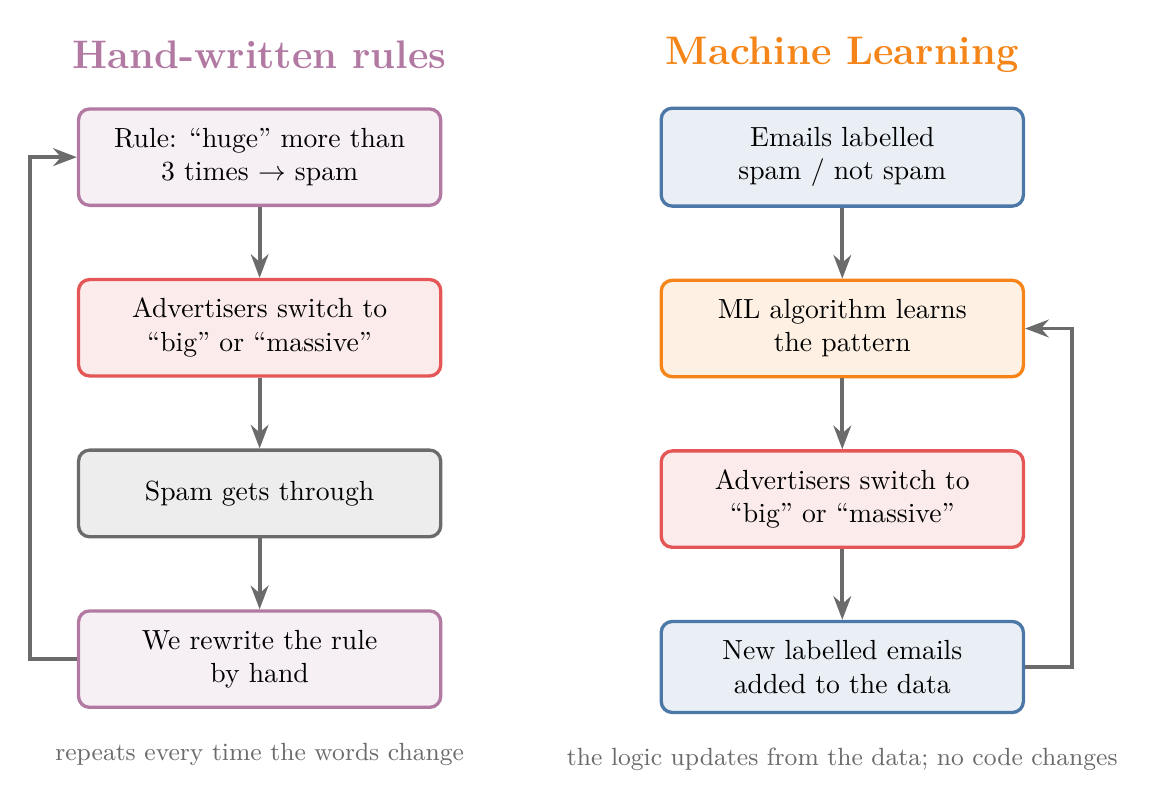
\begin{tikzpicture}[node distance=0.9cm]
  % left: hand-written rules
  \node[title, cpurple] at (2.2,1.3) {Hand-written rules};
  \node[box=cpurple, minimum width=4.6cm] (r1) at (2.2,0) {Rule: ``huge'' more than\\3 times $\rightarrow$ spam};
  \node[box=cred, minimum width=4.6cm, below=of r1] (a1) {Advertisers switch to\\``big'' or ``massive''};
  \node[box=cgrey, minimum width=4.6cm, below=of a1] (m1) {Spam gets through};
  \node[box=cpurple, minimum width=4.6cm, below=of m1] (w1) {We rewrite the rule\\by hand};
  \draw[arrow] (r1) -- (a1); \draw[arrow] (a1) -- (m1); \draw[arrow] (m1) -- (w1);
  \draw[arrow] (w1.west) -- ++(-0.6,0) |- (r1.west);
  \node[note, below=0.3cm of w1] {repeats every time the words change};
  % right: machine learning
  \node[title, corange] at (9.6,1.3) {Machine Learning};
  \node[box=cblue, minimum width=4.6cm] (d2) at (9.6,0) {Emails labelled\\spam / not spam};
  \node[box=corange, minimum width=4.6cm, below=of d2] (t2) {ML algorithm learns\\the pattern};
  \node[box=cred, minimum width=4.6cm, below=of t2] (a2) {Advertisers switch to\\``big'' or ``massive''};
  \node[box=cblue, minimum width=4.6cm, below=of a2] (n2) {New labelled emails\\added to the data};
  \draw[arrow] (d2) -- (t2); \draw[arrow] (t2) -- (a2); \draw[arrow] (a2) -- (n2);
  \draw[arrow] (n2.east) -- ++(0.6,0) |- (t2.east);
  \node[note, below=0.3cm of n2] {the logic updates from the data; no code changes};
\end{tikzpicture}
\end{document}
